\documentclass{beamer}
\mode<presentation> {
\usetheme{Madrid}
}
\usepackage{graphicx}
\usepackage{booktabs}
\usepackage[T2A]{fontenc}
\usepackage{mathtools}
\usepackage[utf8]{inputenc}
\usepackage[english, russian]{babel}
\usepackage{gensymb}
\usepackage{floatrow}
\usepackage{float}
\usepackage{gensymb}
\usepackage{amsmath}
\usepackage{amssymb}

%--------

\title[Лабораторная работа №3.3.1]{Измерение удельного заряда электрона}

\author[]{Голышев Иван и Медведев Илья}
\institute[]{Московский физико-технический институт}
\date{Сентябрь, 2022}

%--------

\begin{document}

%-------1

\begin{frame}
\titlepage
\end{frame}

%-------2


\begin{frame}
\frametitle{Цель работы} 
Определение отношения заряда электрона к его массе методом магнитной фокусировки и методом магнетрона.
\end{frame}

%---------3

\begin{frame}
\frametitle{Метод магнитной фокусировки: теория}
Пусть магнитное поле однородно и постоянно ($\Vec{B}\;=\;const$). Тогда траектории движения заряженных частиц в нем имеют форму спирали, радиус которых описывается:
\begin{equation}
   r_{B} = \frac{v_{\perp}}{\omega_{B}} = \frac{mv_{\perp}}{qB} 
\end{equation}
Откуда найдем шаг спирали за циклотронный период:
\begin{equation}
    T_{B} = \frac{2\pi r_{B}}{v_{\perp}}\;\longrightarrow\;L = v_{\parallel}T_{B} = \frac{2\pi v \cos{\alpha}}{\frac{e}{m} \cdot B},
\end{equation}
где $\alpha$ -- угол между $\Vec{v}$ и $\Vec{B}$.
\end{frame}

%----------4

\begin{frame}
\frametitle{Метод магнитной фокусировки: теория}
При малых углах $\alpha\;\ll\;1, \cos{\alpha} \approx 1:$
\begin{equation}
    L \approx \frac{2\pi v}{\frac{e}{m}B}
\end{equation}
Значит при малых углах $L \neq L(\alpha)$. 
Откуда делается вывод, что \textbf{индукция поля $B$ определяется только удельным зарядом электрона $\frac{e}{m}$.}
\end{frame}

%-----------5

\begin{frame}
\frametitle{Метод магнитной фокусировки: экспериментальная установка и методика эксперимента}
    \begin{wrapfigure}
	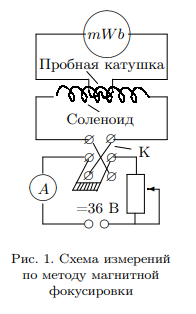
\includegraphics[width=3cm]{ris1.PNG}
	\label{ris:ris1}
    \end{wrapfigure}
\newline
Если расстояние от пушки до экрана l, то пучок сфокусируется на экране при условии
\begin{equation}
    l = nL, где n = 1, 2, 3, . . . ,
\end{equation}


\end{frame}
%--------------6

\begin{frame}
\frametitle{Метод магнитной фокусировки: экспериментальная установка и методика эксперимента}
Скорость движения электрона можно найти, зная разность потенциалов $U_A$, пройденную электроном:
\begin{equation}
    \frac{mv^2}{2} = eU_A\;\longrightarrow\;v_\parallel = \sqrt{\frac{2eU_A}{m}}
\end{equation}
Обозначая $B_f$ -- величину поля при фокусировки пучка электронов, получим:
\begin{equation}
    \frac{e}{m} = \frac{8 \pi^2 U}{l^2} \frac{n^2}{B_f^2(n)}
\end{equation}
\end{frame}

%---------7
\begin{frame}
\frametitle{Метод магнитной фокусировки: ожидания}
\begin{itemize}
    \item Результат $\frac{e}{m}$ должен совпасть с результатом, полученным методом магнетрона,
    \item Калибровочный график $B(I)$ должен быть линейным,
    \item Рассчетный график $B_f(n)$ тоже должен быть линейным.
\end{itemize}
\end{frame}

%------8
\begin{frame}
\frametitle{Метод магнитной фокусировки: обработка результатов}
1. Снимаем зависимость $Ф(I)$. С помощью формулы $Ф = BSN$ получаем зависимость $B(I)$.
\begin{wrapfigure}
	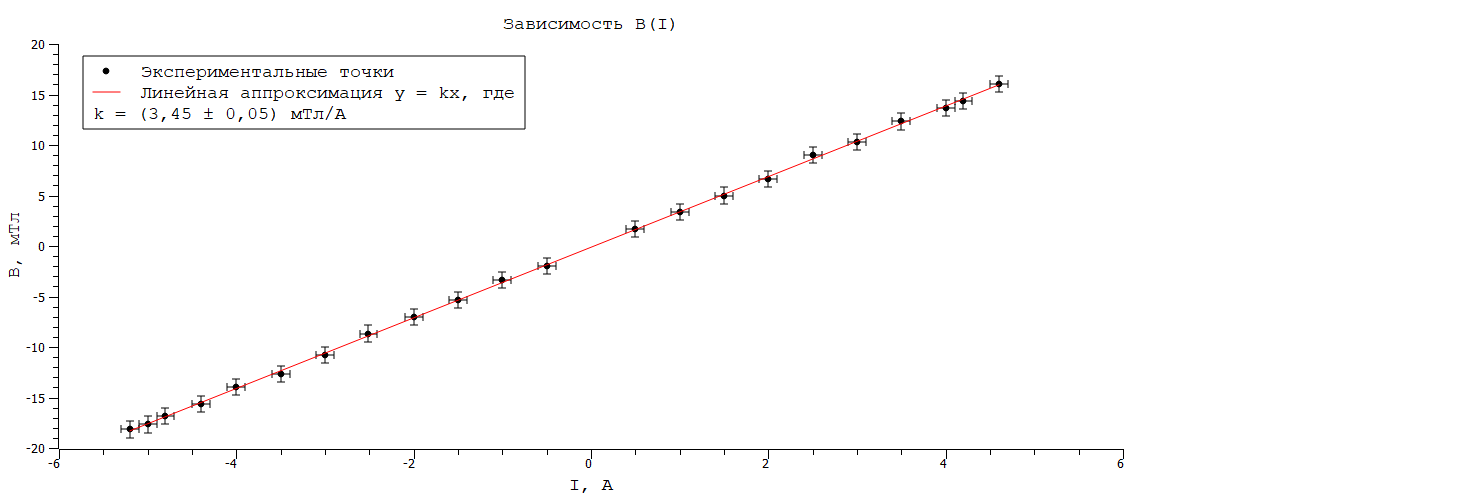
\includegraphics[width=14.5cm]{g2.PNG}
	\label{ris:ris2}
\end{wrapfigure}
\end{frame}
%------9
\begin{frame}
\frametitle{Метод магнитной фокусировки: обработка результатов}
2. Из графика $B(I)$, определяем усредненные значения $B_f$ для каждого фокуса. Строим $B_f(n):$
\newline
\begin{left}
\begin{wrapfigure}

	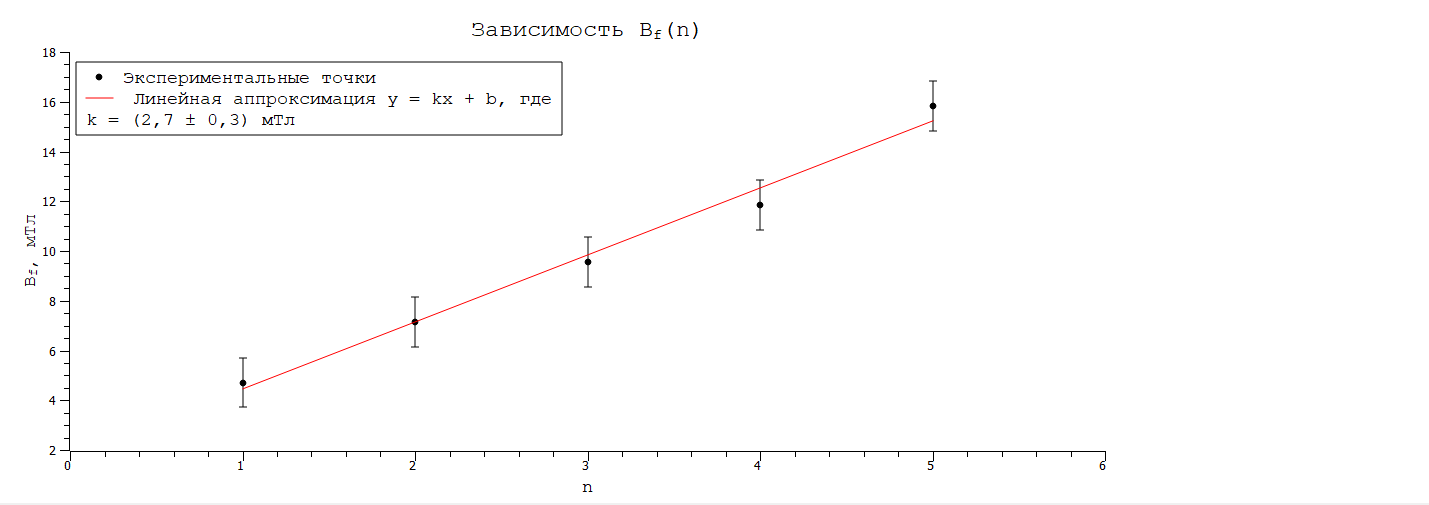
\includegraphics[width=17cm]{g1.PNG}
	\label{ris:ris1}
    \end{wrapfigure}
\end{left}
\end{frame}


%-----10
\begin{frame}
\frametitle{Метод магнитной фокусировки: обработка результатов}
Из графика (2) и формулы (6), получаем:
\[\frac{e}{m} = \frac{8 \pi^2 U}{l^2} \frac{n^2}{B_f^2(n)}\]
\[\longrightarrow \frac{e}{m} = (1,2 \pm 0,4) \cdot 10^{11}\; C/kg\] 
\end{frame}

%------11
\begin{frame}
\frametitle{Метод магнетрона: теория}
В так называемом методе магнетрона отношение e/m измеряется на
основе исследования движения электрона в скрещенных электрическом и магнитном полях, перпендикулярных друг другу.
\begin{wrapfigure}
	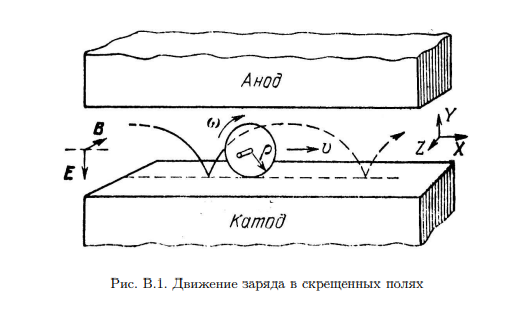
\includegraphics[width=10cm]{ris2.PNG}
	\label{ris:ris2}
\end{wrapfigure}

\end{frame}
%------12
\begin{frame}
\frametitle{Метод магнетрона: теория}
Пусть $\Vec{E} \perp \Vec{B}.$  Тогда 
\begin{itemize}
    \item $\forall U\; \exists B_{cr}: $ траектории электронов касаются поверхности анода.\\
    \item Если $B < B_{cr}$, то все электроны
достигают анода и ток через магнетрон имеет то же значение, что и без
магнитного поля.\\
    \item Если же $B > B_{cr}$, то электроны не достигают анода и
ток через лампу равен нулю.\\

\end{itemize}
\end{frame}

%------13
\begin{frame}
\frametitle{Метод магнетрона: теория}
Рассчет $B_{cr}:$
\begin{equation}
    m\dot{\Vec{v}} = q\Vec{E} + q\Vec{v} \times \Vec{B}
\end{equation}
\begin{equation}
    \longrightarrow \dot{v_x} = \omega_B v_y,\;\;\dot{v_y} = \frac{q}{m}E - \omega_B v_x
\end{equation}
Решение дифф. уравнений -- циклоида:
\begin{equation}
    x = vt - R \sin{\omega t},\;\; y = R(1 - \cos{\omega t}),
\end{equation}
где $v = \frac{E}{B},\; R = \frac{Em}{eB^2}.$ \\
Касание происходит при $2R = h$. Откуда:
\begin{equation}
    B_{cr} = \frac{\sqrt{2U}}{h\sqrt{\frac{e}{m}}} \longrightarrow \frac{e}{m} = \frac{2U}{B_{cr}^2 h^2}
\end{equation}
\end{frame}

%------14
\begin{frame}
\frametitle{Метод магнетрона: экспериментальная установка и методика}
\begin{wrapfigure}
	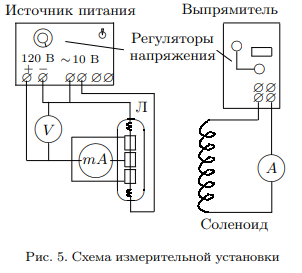
\includegraphics[width=5cm]{ris4.PNG}
	\label{ris:ris2}
\end{wrapfigure}
Движение электронов в этом случае проис
ходит в кольцевом пространстве, заключённом между
катодом
и анодом двухэлектродной электронной лампы (рис. 2). 
\end{frame}


%-------15
\begin{frame}
\frametitle{Метод магнетрона: экспериментальная установка и методика}
\begin{wrapfigure}
	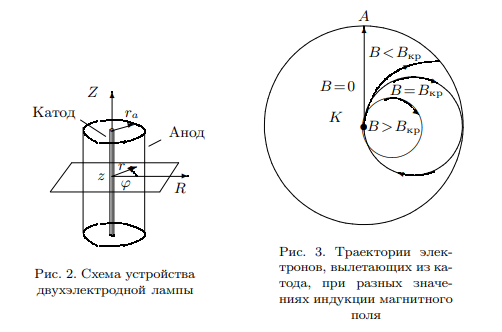
\includegraphics[width=10cm]{ris3.PNG}
	\label{ris:ris2}
\end{wrapfigure}
\end{frame}

%-------16

\begin{frame}
\frametitle{Метод магнетрона: экспериментальная установка и методика}
Пусть потенциал анода равен $U_A$.
Решая задачу о движении электрона в магнетроне, получим, что:
\begin{equation}
    eU = \frac{m}{2} (\dot{r}^2 + (r\frac{eB}{2m})^2)
\end{equation}
При $r = r_a\;\;\dot{r} = 0.$ Откуда:
\begin{equation}
    \frac{e}{m} = \frac{8U_A}{r_A^2B_{cr}^2}
\end{equation}
\end{frame}

%-----17
\begin{frame}
\frametitle{Метод магнетрона: ожидания}
\begin{itemize}
    \item Результат $\frac{e}{m}$ должен совпасть с результатом, полученным методом магнитной фокусировки,
    \item Зависимости $I_M(I_C)$ должны иметь на некотором участке резкий наклон,
    \item Зависимость $B_{cr}^2(U_A)$ должна быть линейной.
\end{itemize}
    
\end{frame}

%-----18
\begin{frame}
\frametitle{Метод магнетрона: обработка результатов}
1. Снимаем зависимость $I_M(I_C)$ для пяти значений $U_A$. Домнажаем $I_C$ на переводной коэффицент $k = 3,5 \cdot 10^{-3}$ (он был написан на установке). Строим семейство кривых $I_M(B):$
\begin{wrapfigure}
	\includegraphics[width=10cm]{п3.jpg}
	\label{ris:ris2}
\end{wrapfigure}
\end{frame}

%-----19
\begin{frame}
\frametitle{Метод магнетрона: обработка результатов}
2. По участкам с резким наклоном графиков определяем $B_{cr}$. Строим график $B_{cr}^2(U_A):$
\begin{wrapfigure}
	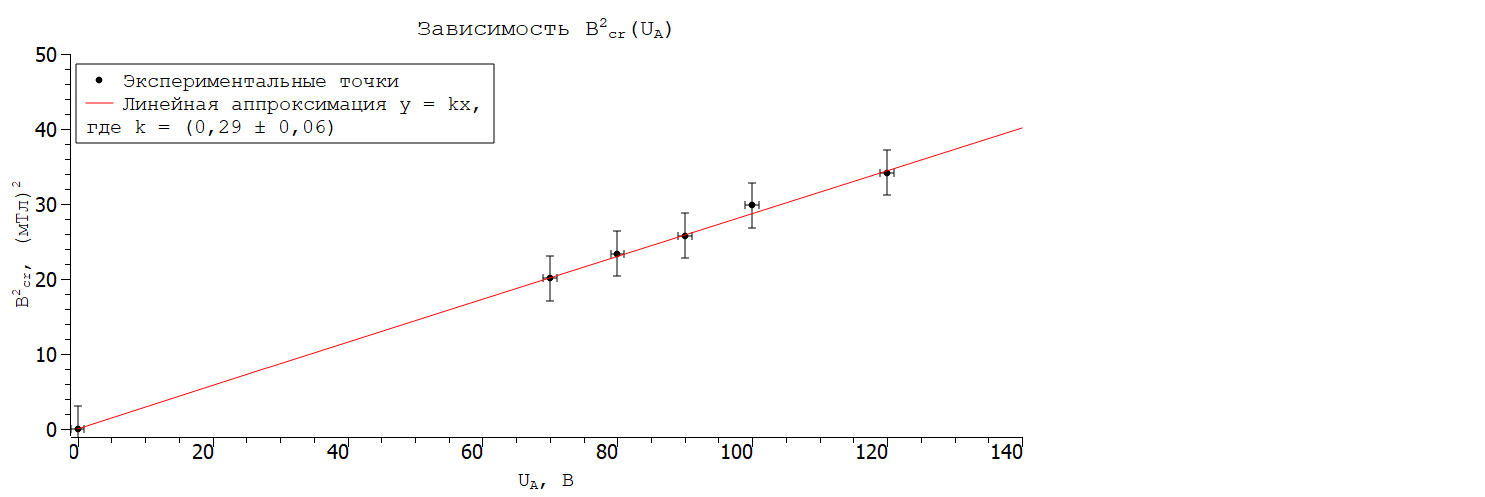
\includegraphics[width=17cm]{g4.PNG}
	\label{ris:ris2}
\end{wrapfigure}
\end{frame}
%-----20
\begin{frame}
\frametitle{Метод магнетрона: обработка результатов}
3. По наклону графика (4) и из формулы (12) получаем:
\[\frac{e}{m} = \frac{8U_A}{r_A^2B_{cr}^2}\]
\[\longrightarrow \frac{e}{m} = (1,9 \pm 0,3) \cdot 10^{11}\; C/kg\]
\end{frame}

%------21
\begin{frame}
\frametitle{Выводы}
\begin{itemize}
    \item $(\frac{e}{m})_{focus} = (1,2 \pm 0,4)\cdot 10^{11}\;C/kg$
    \item $(\frac{e}{m})_M = (1,9 \pm 0,3)\cdot 10^{11}\;C/kg$
    \item $(\frac{e}{m})_{table} = 1,76\cdot 10^{11} \;C/kg$
\end{itemize}
Как мы видим экспериментально полученные значения попадают в $2\sigma$ окрестность эталонного значения.

\end{frame}


%------22
\begin{frame}
\frametitle{Обсуждение результатов}
Недостатки метода магнетрона:\\
В идеальной модели график I(B) должен иметь вертикальный скачок в точке $B_{cr}$, но на практике такой зависимости нет. Авторы считают, что это связано с неоднородностью поля и с тепловым движением электронов. Поэтому уравнение (7) точно не описывает траекторию движения всех электронов.

\end{frame}
\end{document}